\documentclass[dvipdfmx]{bta}

\title{ハニーポットによる不正ファイルの入手と分析}
\author{G984822019}{吉村 直将}
\supervised{
	\supervisor{教授}{蓑原 隆}
	\supervisor{助手}{田島 信行}
}

%\newenvironment{comment}{\color{red}}{\color{black}}

\begin{document}
\maketitle

\chapter{はじめに}
%\subsection{研究背景}
% 近年,サイバー攻撃の発生件数が年々増加してきており,その攻撃手法も多様化している.
% 対策として,攻撃者を誘き寄せ,
% 不正アクセスを受けるハニーポットを運用し,
% 攻撃者の情報を収集してきた.過去の研究では,
% ハニーポットを利用して,
% ログイン試行時に使われるIDやパスワード,
% ログイン後に攻撃者から送られるシェルコマンド等の情報を収集し,研究を行ってきた.
% 得られる情報の中でログイン後に送られるコマンドを解析することは、
% 攻撃者がログイン成功後にどうゆう意図で,何を目的をとして攻撃を行なってくるかの予測が立てらる.
% 又,コマンドから攻撃者がダウンロードさせようとしてくる不正なソフトウェアの情報を知り、調査できる為,
% より最新の攻撃に対して具体的なセキュリティ対策につながると思われる.

近年,サイバー攻撃の発生件数が年々増加してきており,その攻撃手法も多様化して
いる.
多様化した新しい攻撃に対処するためには攻撃手法の分析が必要である.
攻撃手法の分析のために,  
攻撃者を誘き寄せ,
不正アクセスを受けるハニーポットを用いて
攻撃者の情報を収集
する方法がある.
例えば
ハニーポットを利用して,
ログイン試行時に使われるIDやパスワード,
ログイン後に攻撃者から送られるシェルコマンド等の情報を収集
する方法が提案されている\cite{Entry}.

%ハニーポットは,攻撃を受け,攻撃内容を記録する.その攻撃手法を分析することで,
%攻撃への対策を強化することやデータ収集方法を改良することにつながる.



% 本研究では、ログイン後に攻撃者から送られるコマンドに着目する.
% コマンドについて解析することは、
% 攻撃者がログイン成功後にどうゆう意図を持ち,何を目的をとして攻撃を行なってくるかの予測が立てらる.
% 又,コマンドから攻撃者がダウンロードさせようとしてくる不正なソフトウェアの情報を知り、調査できる為,
% より最新の攻撃に対して具体的なセキュリティ対策につながると思われる.

本研究では,より具体的な攻撃者の攻撃手法の情報を得るため,攻撃者がログイン成功後に行う攻撃に着目し,
ハニーポットを用いて,攻撃者から送信されるコマンドやそのコマンドから入手できるファイルの情報を収集し,解析するシステムを構築する.
そして,攻撃の分析を行い,最新の攻撃内容について警告を発することを目的とする.

\chapter{攻撃収集分析システム}


攻撃者がダウンロードさせようとしてくる
不正なソフトウェアの解析を実現する為のシステムの構成を図\ref{fig:system}に示す.

\begin{figure}[htbp]
	\centering
 	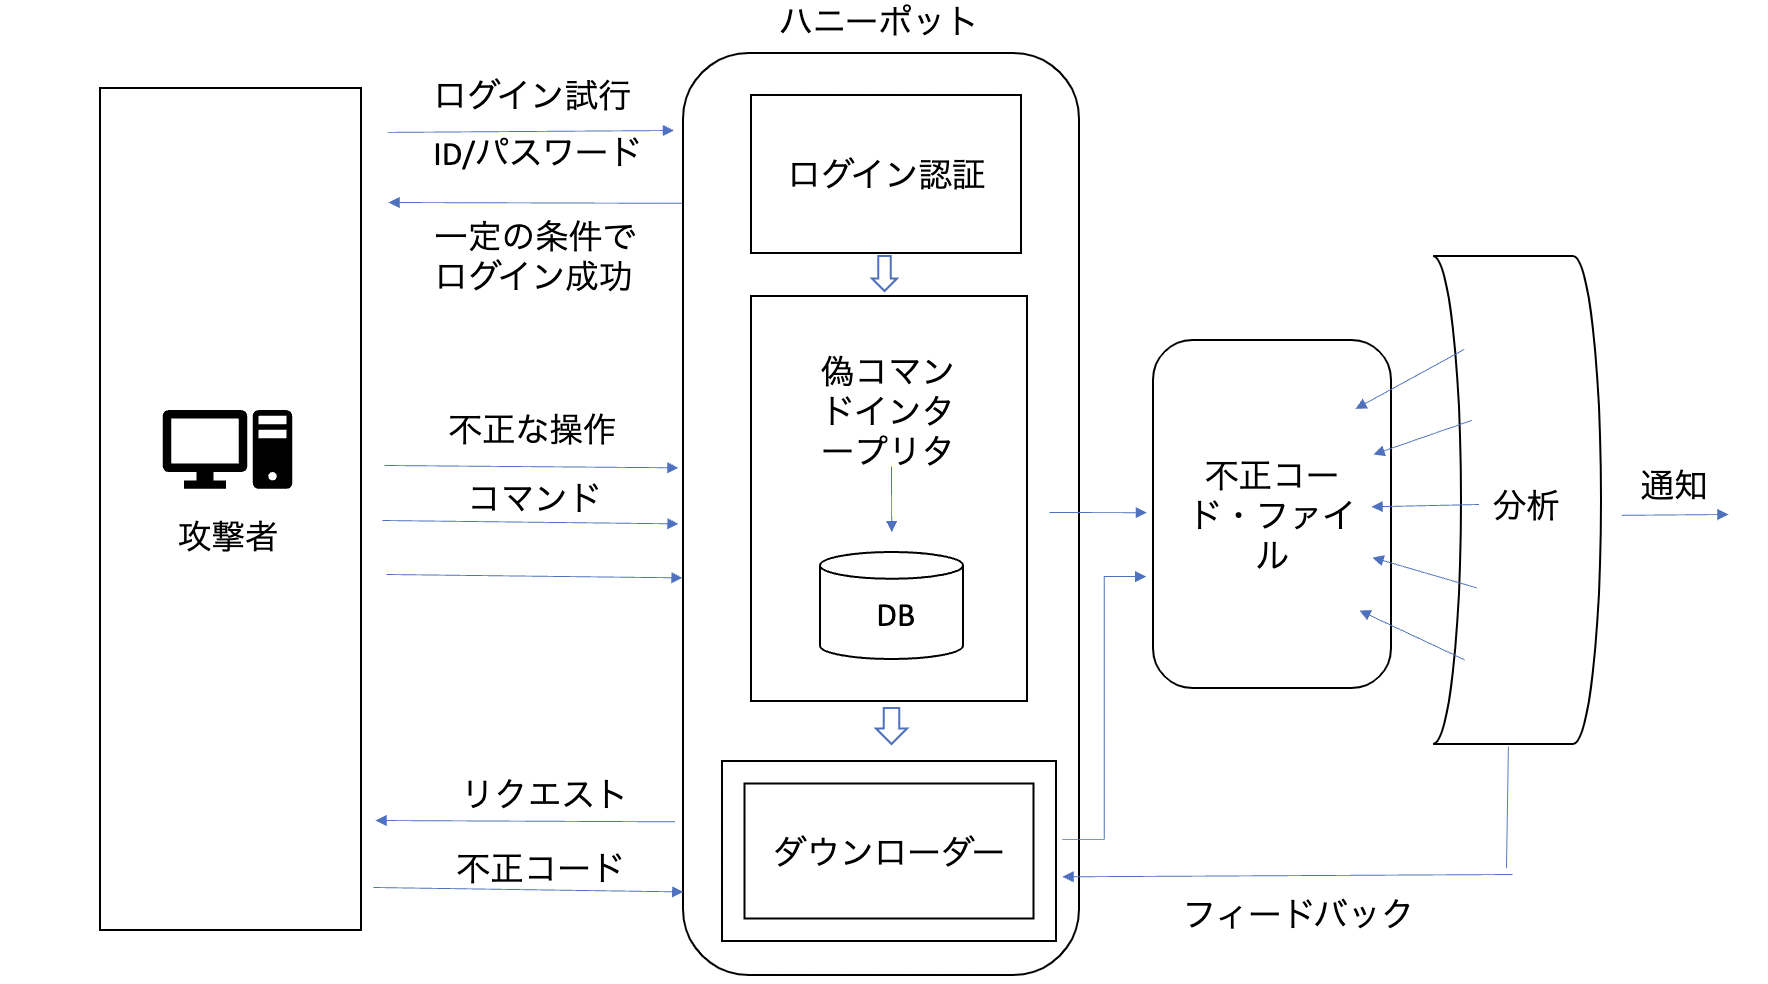
\includegraphics[width=\linewidth]{hpsystem2.png}
 	\caption{システムの構成}\label{fig:system}
\end{figure}


%\subsection{攻撃ホストからハニーポットへの攻撃の流れ}

%攻撃者ホストからハニーポットへの攻撃の流れとして図1に示してある.

% \Repl{攻撃ホスト}{ハニーポット}
% は
% ログイン試行としてID/パスワードを送信してくる
% \Repl{ハニーポットはそれ}{攻撃ホスト}
% に対して,ログイン許可をしている風に見せる.
% \Repl{}{このとき,}ログイン試行時に使われるIDやパスワード
% \Repl{}{を記録する}.

% 攻撃者はログイン\Repl{後}{に成功したシステムを}操作する
% \Repl{為}{ため}に,コマンドを送信する
% \Repl{この攻撃の中でハニーポットはログイン後に}{ので,}
% 攻撃者から送られるシェルコマンド等の情報を収集
% \Repl{し,収集した情報から攻撃手法の研究してきた.}{する}.

ハニーポットは,攻撃者からの何度かのログイン試行を受け,
一定の条件で,攻撃者にログイン成功したと思わせる.
その後,攻撃者にコマンドインタープリタの様な返答を見せ,
不正な操作のコマンドをデータベースDBに収集する.
% 
収集したコマンドから,
攻撃者が不正なサイトから
ダウンロードさせ
ようとする
不正なファイルを安全に入手する.
また,
% コマンドの中には,コマンドからハニーポット内に
% 直接不正なファイルを作成しようとしてくるものもあり,
% 安全にファイルを作成して収集する.
コマンドの中には,ハニーポット内に不正ファイルの作成を試みるものもあり,
安全にファイルを作成し,収集を行う.
% 
収集した不正ファイルのコードから,
どの様な不正ファイルかを分析し警告を発
する.また,
その情報からダウンローダーに生かせるものをフィードバック
する.
% 
% \begin{figure}[htbp]
% 	\centering
% 	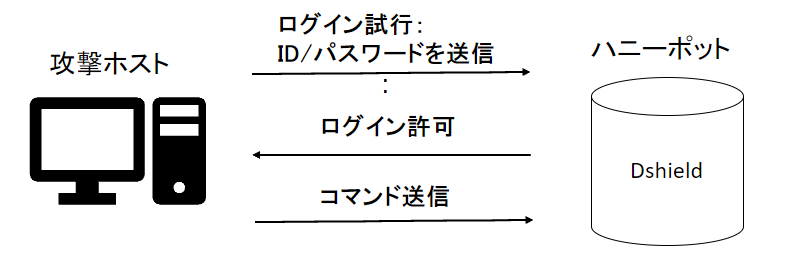
\includegraphics[width=\hsize]{honeypot1.png}
% 	\caption{攻撃の流れ}
% \end{figure}

%\subsection{目的}

% 本研究では,ハニーポットDshieldを用いる.DShield(Distributed Intrusion Detection System)は,
% グローバルなセキュリティコミュニティによって構築された分散型侵入検知システムである.
% 世界中のネットワーク上で発生するセキュリティイベントのデータを収集し,
% 分析することでセキュリティの脅威情報を提供する.Dshieldは研究室で以前から運用していたが,
% ログイン試行時のIdやパスワードを収集することを目的としたハニーポットであった.
% 本研究では,ログイン後のコマンドを収集することが目的としている為,
% 新しくハニーポットを構築することとする.                

%\subsection{システムの実装}

本研究では,ハニーポットとしてDShield
(Distributed Intrusion Detection System)\cite{DShield}
と呼ばれるグローバルなセキュリティコミュニティによって構築された分散型侵入検知システム
を使用する.
% 本研究でのハニーポットの実装は,Dshield
% と呼ばれる
% グローバルなセキュリティコミュニティによって構築された分散型侵入検知システム
% をベースに開発を行う.
%世界中のネットワーク上で発生するセキュリティイベントのデータを収集し,
%分析することでセキュリティの脅威情報を提供する.
これまで我々の研究室では主に
攻撃頻度の時系列解析のために
Dshieldハニーポットを利用している\cite{nishida2022}.
が,本研究では図\ref{fig:system}に示すように,Dshieldのcowrie\cite{Cowrie}のログイン認証部,コマンドインターポリタ部に必要な機能を追加する,
また,コマンドからファイル又は,URLなどを取集する
ダウンローダー部,
不正ファイルの分析部は,新しく
プログラムを作成する.
% 研究計画として,
% \begin{enumerate}
%     \item Dshieldを運用できる環境を構築をする.
%     \item コマンドを収集するために、Dshieldのプログラム内で、
% 	攻撃者からのコマンドに対してどのような動作をしているかを確認する.
%     \item 実際にDshieldを運用してみる.
%     \item取集したコマンドの内容について調べる.
%     \item 
%     \item ファイルがどのようなものなのか調べる.
% \end{enumerate}
% という手順で進めていき,攻撃ファイルがどの様なものなのか把握し,
% どのような対策が有効的なのか等の警告を発することで,セキュリティの向上に貢献していく.

%\section{進捗状況}
\chapter{Dshiledの環境構築と運用}

Raspberry PiにDshieldをインストールし,パスワードや接続する無線LANの設定を行なった.
Rassberry Piのファイアウォールの設定からSSHを有効にする事で,
外部からの接続をcowrieが対応するように設定した.
また,研究室内のネットワークからの接続は攻撃と見さないように設定した.

%\subsection{Dshieldが行う攻撃者のログイン試行への対処方法}

%Dshieldは研究室で以前から運用されていたがidやパスワードの収集を目的として使われていた.
攻撃者から
コマンドを収集
するために
Dshieldのプログラム
を調査し,
コマンドを収集できているのか確認した.
まず初めに,Cowrieは,攻撃者からのコマンドをどう対処しているのかを調べ,t攻撃者に返すコマンドのディレクトリとしてextcomsファイルがあることが分かった.次に,このファイルを使っているものを次のコマンドで検索し,
\verb!find. -exec grep, textcmds {}\; -and -print 2 > /dev/null!
srv/cowrie/shell/protocol.pyで使われていることが分かった.
調査の結果,Dshieldは
攻撃コマンドを取集し,
/srv/cowrie/var/log/cowrieの場所に保存
していることが分かった.
また,ログイン試行に対応しているプログラムが
/src/cowrie/core/の場所にあるauth.pyである
ことを突き止め,解読したところ,
Dshieldは外部からの攻撃者
%(一つの決まったIPアドレス)
からのログイン試行を1回以上のランダム数行うと,
ログイン可能とする
ように設定されていることが
分かった.

% そのログイン成功時に使用していた
% ユーザーIDとパスワードがそのIPアドレス限定でのログイン成功するものとなる.
% これは,ハニーポットと見破られないように考えられたシステムだと思われる.

%\subsection{収集したコマンド内容と攻撃者の意図}
実際にハニーポットを運用し5/19から5/30の期間中にコマンドを取集した.
収集したコマンドの中には
特定のパターンのコマンドが多く発見された.
例えば組み込みLinuxで複数のコマンドをまとめるために使われる
busyBoxが含まれていて,
この期間中に多くの攻撃が組み込みLinuxの機器を対象としていることが分かった.
また,収集したコマンド中には,不正なファイルをダウンロードさせるためwgetコマンドを用いているものや,
不正なファイルをハニーポット内に作成するために,echoコマンドを用いているものが多かった.

\chapter{ダウンローダー部の作成}
ダウンローダー部のシステムプログラムは,主に3つの動作を行う.

\renewcommand{\labelenumi}{(\arabic{enumi})}
\begin{enumerate}
	\item 不正ファイルデータのダウンロードコマンドを模倣して不正データを入手する
	\item 不正データを安全に扱うためにヘッダ情報を追加する
	\item データを保存するファイル作成し,ヘッダ情報と不正ファイルデータを書き出す.
\end{enumerate}

(1)について,
Dshieldでの攻撃コマンドを模倣している部分を調査し,
srv/cowrie/src/cowrie/commandsの下にPythonプログラムとして実現されていることが分かった.
例えば,不正ファイルデータのダウンロードに使われているwgetの動作は,wget.py中で行われる.主なそのファイル内の動作プログラムとして,123行目の
\verb!self.deferred = self.download(self.url, self.outfile)!で不正サイト情報であるdefeerredを,引数としてURLとoutファイルでdownload関数によって取得する.124から128行内の
\verb! if self.deferred:!のif文で不正サイト情報が得られたら\verb!self.deferredaddCallback(self.success)!successメソッドへ移動し,上手く得られなかったら\verb!self.deferred.addErrback(self.error, self.url)!でerrorメソッドへ行く.そして,successメソッド内で(2)と(3)の処理を行うコードを追加した.

(2)において,
ヘッダ情報を不正データに追加するのは,
ダウンロードしたデータをそのままファイルとして保存することを避け,不正データのファイルを誤って動作させてしまった場合でも問題が起きないようにする
安全対策のためである.
具体的なヘッダ情報としては,ダウンロードに使用したURLの前に4桁のURL文字数を追加したものとし,URLの文字数は,4桁の数字を追加したものとする.プログラムとしてURLの文字数は,formatメソッドを利用し,0埋めを行う.\verb!hd = '{:04}'.format(hdct)!.

(3)については,
Dshieldハニーポットが攻撃者に見せているファイルシステムの外の領域として外付けHDDに作成する,そしてファイル名とするfnameは,ファイル場所と攻撃があった日時を入れ,

\verb!fname = "/HD/malwares/tmp/MW" + str(now.date()) + "_" + str(now.time())!,
open関数でファイルを作成する.\verb!self.file = open(fname, "wb")!.
%Dshieldハニーポットが攻撃者に見せているファイルシステムの外の領域に,攻撃があった日時を追加した名前のファイルを作成する.

実際に研究室で運用しているハニーポットに組み込んで確認したところ,攻撃があったときにデータが記録されていないことが判明した.原因はDShieldが1日に1回,18時28分に,配布元を確認し,システムのアップデートがあった時,自動的に更新しているためであった.そこでハニーポットの/etc/cron.d/dshieldにアップデートの情報が持ち,そのファイルをwget.pyへ周期的に変更を加えたもので上書きをするように設定し,正しく動作していることを確認した.

\chapter{不正ファイルの分析}
不正ファイルの分析として実際の不正ファイルからの情報取得を行った.
具体的には,直接不正ファイルを作成させようとしてくる攻撃の 1 つとして,
複数の echo コマンド を次のように送るものについて,
\verb!echo -ne "\x7f\x45.." > niggabox!
実際にファイルを作成して調査した.以下,作成したファイルを対象データと呼ぶ. 
まず,対象データは2,720バイトのバイナリーデータであることがわかった.
バイナリーデータのファイルは,最初の数バイトがファイル形式を示している場合が多い.対象データについて先頭部分を調べたところ,
最初の4バイトが,“x7f x45 x4c x46” であり,ELF形式\cite{elf}のファイルであると判別した.

次にELF形式のヘッダ情報の解析を行う.ELF形式のファイル構造では,具体的に,1から4バイトがファイル形式を示し,5バイト目が32or64ビットのファイルか.6バイト目がリトルエンディアンかビックエンディアン方式か,18バイト目が対象としているアーキテクチャの種類,と判別することができる.そのため,今回の対象データは,32ビットのリトルエンディアン形式で,ARMアーキテクチャ用であることがわかった.そこで,次のコマンドで逆アセンブリを行い,
\verb!objdump --print-imm-hex!
--disassemble -s niggabox!
内容を確認したところ,マルウェアのMiraiのソースコード\cite{Mirai}として公開されているコードの一部に酷似していた.さらに,リンク先から別のファイルをダウンロードする機能を持っていることが分かり.具体的にこの不正ファイルでは,リンク先はアムステルダムで,別のファイルはjklarmというファイルであることも分かった.


%不正ファイルの分析に伴い,初めに実際の不正ファイルから具体的に何の情報が得られるかを調べた.
%まず,直接不正ファイルを作成させようとしてくる攻撃コマンドの1つである echo -ne "\x7f\x45.." > niggabox を
%利用し,そこから得られる不正ファイルデータから調べた.
%ファイルのバイナリーデータは,最初の数バイトがファイル形式を示している.
%その為,最初の数バイトでファイル形式を判別する.
%今回得られた不正ファイルデータの一つは,最初の4バイトが"x7f x45 x4c x46”であることから,
%ELF形式のファイルであると判別できた.
%また,ファイル形式の種類によって構造は主に決まっていることから,
%その形式の構造からファイルの情報を取得できる.
%よって,ELF形式のファイル構造を調査する.

\section{ELF形式のファイルから情報取得の自動化}
ELF形式のファイルについて,自動で情報を解析するためのプログラムを作成した.ELF形式は図2に示すように,実行時にメモリ上に展開される.text,.rodataなどの複数セクションで構成されている.セクションは,ELFヘッダ,プログラムヘッダテーブル,セクションヘッダテールの3種類あり,ELFヘッダでは,プログラムヘッダテーブルとセクションヘッダテーブルのサイズやオフセットの情報が取得できる.また,プログラムヘッダテーブルでの情報で,読み出し可能なデータのセグメントに分けられている.各セクションの境界はセクションヘッダテーブルの情報で切り分けられる.
\begin{figure}[htbp]
	\centering
 	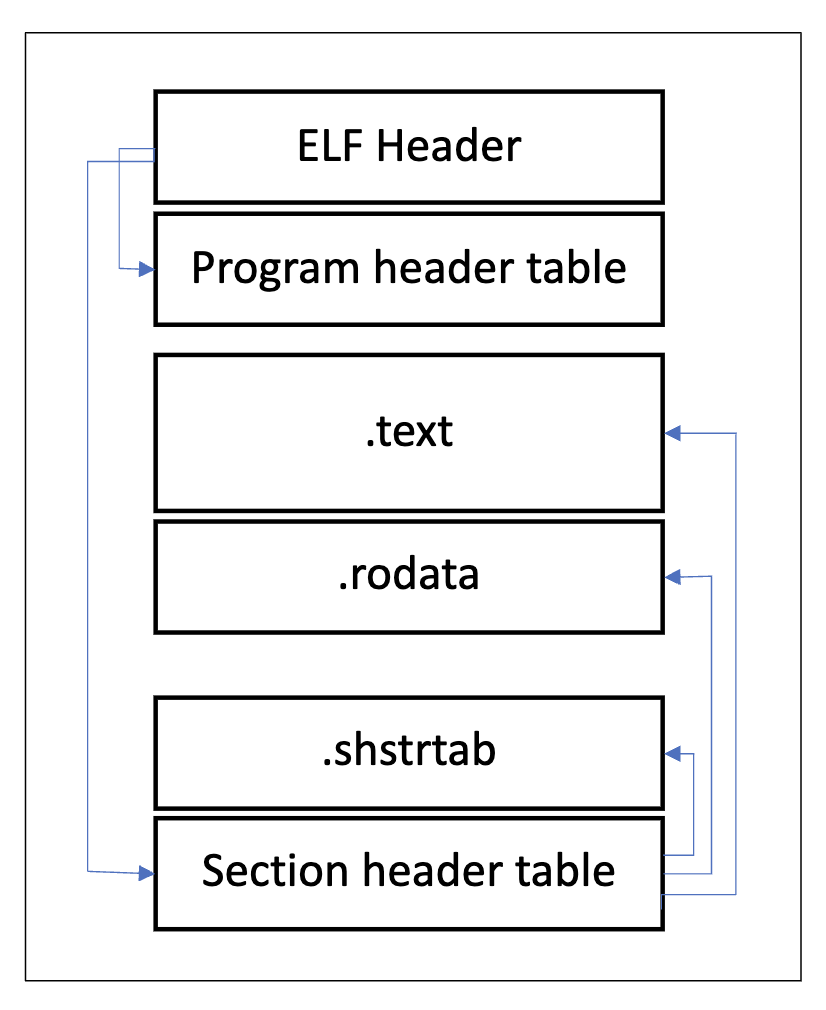
\includegraphics[width=\linewidth]{elf.png}
 	\caption{ELF形式のファイル構造}\label{fig:system}
\end{figure}

自動情報取得として,プログラムに埋め込まれた文字列などのリテラルが格納されている.rodataから情報を取得する処理を実装した.ELF形式では各セクションが記録される順番は規定されていないが,各セクションの名前のテーブルが格納されたセクション(.shstrtab)からの番号はELFヘッダから取得できる.セクションヘッダテーブルは,エントリという項目で分かれており,各エントリは一つ一つのセクションの情報について書かれている.各エントリ内の一部が.shstrtabセクションのテーブルの番号の情報をもつため,その番号で各エントリがどのセクションかを判断ができる,そこで,.rodataを検索し,対応するセクションの内容をダンプするようにプログラムした.
手作業での分析に使用した対象データ(niggabox)について,作成したプログラムを実行し,図3のようにダウンロードしようとするファイル名(jklarm7m)などの情報が取得できることを確認した.
また,このプログラムを応用して,
%ELF形式のファイル構造は,複数のセクションから構成されている.
%その中に3つのヘッダとして,ELFヘッダ,プログラムヘッダ,セクションヘッダがあり,
%主にヘッダは各セクションについての情報を持っている.
%ELFヘッダは,他2つのヘッダ情報を持っており,大きさや位置情報が取得できる.
%また,セクションヘッダでは,各セクションごとに何の情報を持っているか等が分かる.
%その為,この二つのヘッダを利用して,どういった情報を持っているかの判別を行う.
%また,セクションヘッダ内は,エントリという項目で分かれていて.
%各エントリは,セクション一つ一つに対応して,
%そのセクションがどういったプログラムやデータかや,サイズやオフセット等の情報を持っている
%また,セクションの一つに,各セクションの名前が羅列された.shstrtabがある.
%こののセクションを利用し,各エントリが
%.shstrtab内にあるセクション名への位置情報を持っていることから、
%対応付けし,各セクションの名前を知ることができる.
%このような形でelf形式の構造からどういったファイル情報を取得すること可能かが分かった.

\chapter{まとめ}

本研究では,Dshieldハニーポットに機能を追加することで,攻撃コマンドが送り込もうとしている不正データを所得し,ELF形式の場合に解析を行うシステムの開発を行なった.我々の研究室で運用しているハニーポットに実装して,不正データの取得および解析結果の表示を行えることを確認した.しかし,解析結果を管理者に通知する部分は未実装で残された課題となっている.

%\bibliographystyle{entry}
\bibliographystyle{ipsjunsrt}
\bibliography{sample}

\end{document}
